\documentclass[en,boletin]{uah}


\tema{3}
\titulo{Efectos del ruido en las comunicaciones analógicas}{Effects of noise in analog communications}
%
\begin{document}

\titulacion{Grados TIC}
\asignatura{Teoría de la Comunicación}{Communication Theory}
\departamento{Teoría de la Señal y Comunicaciones}
\curso{2024/2025} % Do not show year

\maketitle

\seccion{Conceptos a repasar}{Key concepts}
\texto{
Antes de hacer estos ejercicios es importante repasar y tener claros los siguientes conceptos teóricos:

\begin{itemize}
\item Esquema general de un sistema de comunicaciones analógico con ruido.
\item Concepto de relación señal a ruido. Diferencia entre predetección y postdetección.
\item Concepto de efecto umbral y cuándo es necesario tenerlo en cuenta.
\end{itemize}
}
{
	Before doing these exercises it is important to review and understand the following concepts:	

	\begin{itemize}
		\item General diagram of an analog communication system with noise.
		\item Concept of signal to noise ratio. Difference between pre-detection and post-detection.
  		\item Concept of threshold effect, and when it is necessary to take it into account. 
	\end{itemize}
}

%%%%%%%%%%%%%%%%%%%%%%%%%%%%%%%%%%%%%%%%%%%%%%%%%%%%%%%%
%%%%%%%%%%%%%%%%%%%%%%%%%%%%%%%%%%%%%%%%%%%%%%%%%%%%%%%%
\seccion{Problemas básicos}{Basic problems}
%%%%%%%%%%%%%%%%%%%%%%%%%%%%%%%%%%%%%%%%%%%%%%%%%%%%%%%%
%%%%%%%%%%%%%%%%%%%%%%%%%%%%%%%%%%%%%%%%%%%%%%%%%%%%%%%%
\texto{
	Este primer bloque de problemas son problemas extraídos en su mayoría de la bibliografía de la asignatura, y consisten en algunos cálculos básicos que es necesario dominar.

}
{
	This first part includes problems mostly extracted from the bibliography aimed at practicing basic calculations needed for the rest of the lesson.

}



\Problema{
	\cite{Carlson} Una señal DBL se demodula utilizando un detector síncrono. Calcula la relación señal a ruido en postdetección en dB sabiendo que la potencia recibida son $20 \textrm{nW}$, el mensaje tiene un ancho de banda de $5 \textrm{MHz}$ y el canal introduce ruido con $N_0 = 4\cdot 10^{-20}$ W/Hz.
}
{
	$\left ( \frac{S}{N} \right )_D = 50 \textrm{ dB}$
}
{
	\cite{Carlson} A DSB signal plus noise is demodulated by synchronous detection. Find $(S/N)_D$ in dB given that the received power is $20 \textrm{nW}$, the message has a bandwidth of $5 \textrm{MHz}$ and the channel introduces a noise with $N_0 = 4\cdot 10^{-20}$ W/Hz.
}
{
	$\left ( \frac{S}{N} \right )_D = 50 \textrm{ dB}$
}


\Problema{
	\cite{Carlson} Una señal DBL se demodula con un detector síncrono con un error de fase $\phi$. Supongamos que el oscilador local tiene la expresión $2 \cos (\omega_c t + \phi)$. Demostrar que $(S/N)_D = \gamma \cos^2(\phi)$.
}{
	
}{
	\cite{Carlson} A DSB signal plus noise is demodulated by a product detector with phase error $\phi$. Take the local oscillator signal to be $2 \cos (\omega_c t + \phi)$ and show that $(S/N)_D = \gamma \cos^2(\phi)$.
}{

}

\Problema{
	\cite{Carlson} Un sistema AM con detección de envolvente está trabajando justo en el umbral. Calcula la ganancia en dB necesaria en el transmisor para conseguir ahora una $(S/N)_D$ de $40 \textrm{dB}$ suponiendo una modulación de un tono puro al $100\%$.

}{
	$\textrm{G} = 32 \textrm{dB}$
}{
	\cite{Carlson} An AM system with envelope detection is operating at the threshold point. Find the power gain in dB needed at the transmitter to get up the $(S/N)_D$ to $40 \textrm{dB}$ with full-load tone modulation.
}{
	$\textrm{G} = 32 \textrm{dB}$
}


\Problema{
	\cite{Carlson} Una señal FM tiene una potencia en recepción de $1 \textrm{nW}$, $W_x = 500 \textrm{kHz}$, $S_{xn} = 0.1$, $|x(t)|_{max} = 4\textrm{V}$, $\omega_d = 500 \textrm{kHz/V}$ y $N_0 = 4\cdot 10^{-20} \textrm{W/Hz}$. Calcula la relación señal a ruido en postdetección de dB para el caso sin filtro de preénfasis y para el caso de utilizar un filtro de preénfasis con $B_{de} = 5 \textrm{kHz}$.

}{
	\begin{itemize}
		\item FM: $(S/N)_D = 53.8dB$
  		\item FM con preénfasis: $(S/N)_D = 69dB$
	\end{itemize}
}{
	\cite{Carlson} An FM signal plus noise has a received power of $1 \textrm{nW}$, $S_{xn} = 0.1$, $|x(t)|_{max} = 4\textrm{V}$, $\omega_d = 500 \textrm{kHz/V}$ and $N_0 = 4\cdot 10^{-20} \textrm{W/Hz}$. Find $(S/N)_D$ in dB for FM detection and for deemphasized FM detection with $B_{de} = 5 \textrm{kHz}$.
}{
	\begin{itemize}
		\item FM: $(S/N)_D = 53.8dB$
  		\item deemphasized FM: $(S/N)_D = 69dB$
	\end{itemize}
}


\Problema{
	\cite{Carlson} Un sistema de comunicaciones analógico tiene $S_x = 1/2$, $W_x = 10 \textrm{kHz}$, $N_0 = 10^{-15} \textrm{W/Hz}$ y unas pérdidas de transmisión de $100 \textrm{dB}$. Calcula la potencia transmitida necesaria para conseguir una relación señal a ruido de postdetección de $40 \textrm{dB}$ para los siguientes casos:

	\begin{enumerate}
		\item AM con $m=1$
  		\item AM con $M=0.5$
    	\item FM con $D = 1$
		\item FM con $D = 5$
		\item FM con $D = 10$
	\end{enumerate}
	
}
{
	\begin{enumerate}
		\item $P_T= 3 \textrm{kW}$
  		\item $P_T= 9 \textrm{kW}$
    	\item $P_T= 667 \textrm{W}$
		\item $P_T= 26.7 \textrm{W}$
		\item $P_T= 24 \textrm{W}$
	\end{enumerate}
}{
	\cite{Carlson} An analog communication system has $S_x = 1/2$, $W_x = 10 \textrm{kHz}$, $N_0 = 10^{-15} \textrm{W/Hz}$, and transmission loss $100 \textrm{dB}$. Calculate the transmitted power needed to get $(S/N)_D = 40 \textrm{dB}$ when the modulation is:

	\begin{enumerate}
		\item AM with $m=1$
  		\item AM with $M=0.5$
    	\item FM with $D = 1$
		\item FM with $D = 5$
		\item FM with $D = 10$
	\end{enumerate}
}{
	\begin{enumerate}
		\item $P_T= 3 \textrm{kW}$
  		\item $P_T= 9 \textrm{kW}$
    	\item $P_T= 667 \textrm{W}$
		\item $P_T= 26.7 \textrm{W}$
		\item $P_T= 24 \textrm{W}$
	\end{enumerate}
}




%%%%%%%%%%%%%%%%%%%%%%%%%%%%%%%%%%%%%%%%%%%%%%%%%%%%%%%%
%%%%%%%%%%%%%%%%%%%%%%%%%%%%%%%%%%%%%%%%%%%%%%%%%%%%%%%%
\newpage
\seccion{Problemas adicionales}{Aditional problems}
%%%%%%%%%%%%%%%%%%%%%%%%%%%%%%%%%%%%%%%%%%%%%%%%%%%%%%%%
%%%%%%%%%%%%%%%%%%%%%%%%%%%%%%%%%%%%%%%%%%%%%%%%%%%%%%%%
\texto{
	Estos problemas son algo más elaborados que los anteriores, en muchos casos extraídos de exámenes antiguos.

}
{
	These problems are slightly more ellaborated than the previous ones, in many cases extracted from old exams.

}




\Problema{

Se dispone de un transmisor que puede modular la señal de entrada en DBL o en AM. Para que el enlace cumpla las especificaciones de calidad, la relación señal a ruido de postdetección debe ser como mínimo de $20 dB$.
	
Cuando se modula en DBL, se consigue un alcance máximo de $15 km$ con una potencia de $1 W$ a la salida del transmisor. La atenuación del enlace (en dB) es proporcional a la distancia que media entre el transmisor y el receptor. 

Se pide:

\begin{enumerate}
	\item Calcular la potencia de la señal a la salida del transmisor cuando modula en DBL y se desea un alcance de $20 km$.
	\item Repetir el apartado anterior en el caso de modulación AM al $80 \%$.
	\item Calcular las potencias de pico de envolvente a la salida del transmisor en las condiciones de los apartados anteriores.
\end{enumerate}
	
\textsc{Datos:}
\begin{itemize}
	\item $\frac{N_0}{2} = 2 \cdot 10^{-9} W/Hz$
	\item $W_x = 2\pi \cdot 5 krad/s$
	\item $|x(t)|_{max} = 1V$
	\item $S_x = 0.5 W$
	\item $\alpha_t[dB] = A \cdot d[km]$, con $A$ constante.
\end{itemize}
	}
	{
		\begin{enumerate}
			\item $S_{T_{DBL}} = 7.96W$
			\item $S_{T_{AM}} = 32.69W$
			\item $PEP_{DBL} = 15.92W$, $PEP_{AM} = 80.25W$
		\end{enumerate}
	
	}
	{

A transmitter can perform either DSB or AM modulations. The post-detection signal-to-noise ratio has to be at least $20 dB$ in order to meet the required quality specifications.

When DSB modulation is used, we get a maximum range of $15 km$ with a transmission power of $1 W$. The link attenuation (in dB) is proportional to the distance between transmitter and receiver. 

Answer:

\begin{enumerate}
	\item Calculate the power of the signal at the output on the transmitter when DSB modulation is used, and the desired range is $20 km$.
	\item Repeat a. when AM at $80 \%$ is used.
	\item Calculate the envelope peak power values at the output of the transmitter under the conditions mentioned in a. and b., respectively.
\end{enumerate}
	
\textsc{Data:}
\begin{itemize}
	\item $\frac{N_0}{2} = 2 \cdot 10^{-9} W/Hz$
	\item $W_x = 2\pi \cdot 5 krad/s$
	\item $|x(t)|_{max} = 1V$
	\item $S_x = 0.5 W$
	\item $\alpha_t[dB] = A \cdot d[km]$, with $A$ a constant.
\end{itemize}
	}
	{
		\begin{enumerate}
			\item $S_{T_{DBL}} = 7.96W$
			\item $S_{T_{AM}} = 32.69W$
			\item $PEP_{DBL} = 15.92W$, $PEP_{AM} = 80.25W$
		\end{enumerate}
	
	}

\newpage

\Problema{

	Una señal normalizada de ancho de banda $5 kHz$ y potencia media $0.5 W$ se transmite en un sistema de modulación AM, siendo la potencia de transmisor de $660 W$. En el receptor, situado a una distancia de $40km$ se obtiene una relación señal a ruido de postdetección de $33 dB$.
	
	Sabiendo que la densidad espectral de potencia de ruido es  $N_0/2=5\cdot 10^{-13} W/Hz$ y que la atenuación de propagación viene dada por $A [dB] = 40+20\cdot log(d[km])$. Se pide:
	
	\begin{enumerate}
		\item El índice de modulación $m$.
		\item La potencia invertida en transmitir la portadora, y la invertida en transmitir cada una de las bandas laterales.
	\end{enumerate}
}
{
\begin{enumerate}
	\item $m=0.8$
	\item $P_p = 500W$, $P_{BL} = 80W$
\end{enumerate}

}
{

	A normalized signal with $5 kHz$ bandwidth and average power $0.5 W$ is transmitted by an AM system. The transmitter power is $660 W$. At the receiver side, located $40 km$ away, we get a post-detection signal-to-noise ratio of $33 dB$.
	
We know that the noise power spectral density is $N_0/2=5\cdot 10^{-13} W/Hz$, and that the propagation attenation is given by $A [dB] = 40+20\cdot log(d[km])$. Answer:

	\begin{enumerate}
		\item Calculate the modulation index $m$.
		\item Calculate the amount of power needed to transmit the carrier, and the amount of power devoted to the transmission of each sideband.
	\end{enumerate}
}
{
\begin{enumerate}
	\item $m=0.8$
	\item $P_p = 500W$, $P_{BL} = 80W$
\end{enumerate}

}


\newpage

\Problema{
	La señal $x(t)$ de la figura se pasa a través de un filtro paso bajo de ancho de banda $10 kHz$, no influyendo esta limitación de banda en la potencia de la señal, y se elimina su componente continua.
	
	{\begin{figure*}[h!]\centering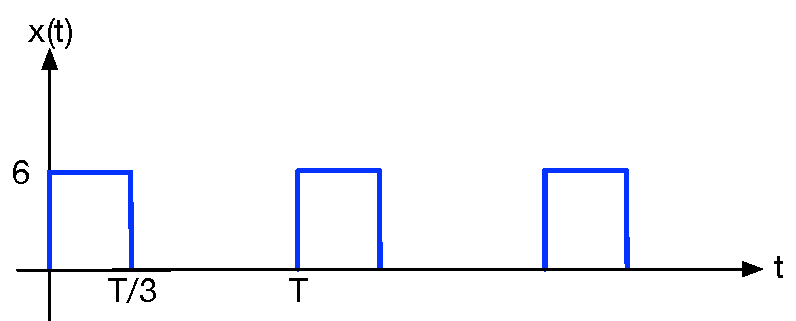
\includegraphics[width=6cm]{./Figuras/Problema3_3a}\end{figure*}}
	
	La señal resultante modula en AM a una portadora de $125 V$. con un índice de modulación de $0.7484$ y se transmite a través de una emisora de radio. El canal de transmisión introduce una atenuación de 80 dB y ruido blanco gaussiano cuya densidad espectral de potencia es $N_0/2=10^{-11} W/Hz$.
	
	Un vehículo que tiene sintonizada esta emisora, penetra en un túnel en cuyo interior la atenuación de propagación deja de ser constante y varia con la distancia según la ley:

\begin{displaymath}
	A[dB] = a_0 + a_1 \cdot d
\end{displaymath}

donde:
\begin{itemize}
	\item $a_0 = 10dB$
	\item $a_1 = \frac{1}{3} dB/m$
	\item $d$: Distancia (m)
\end{itemize}

{\begin{figure*}[h!]\centering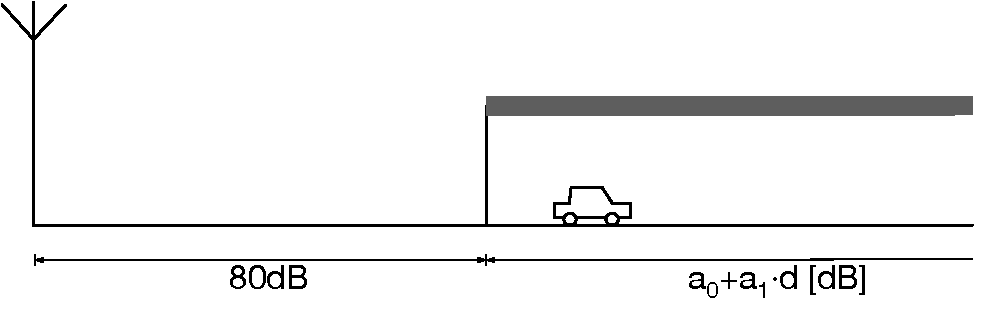
\includegraphics[width=8cm]{./Figuras/Problema3_3b}\end{figure*}}

Se pide:

	\begin{enumerate}
		\item Obtener la potencia media de la señal modulada.
		\item Obtener la relación señal a ruido de demodulación a la entrada del túnel.
		\item Obtener la distancia a la que dejará de oírse la señal, en el vehículo, sabiendo que el umbral de demodulación del coche es de $10 dB$.
		\item Repetir el apartado anterior si el demodulador utilizado es un detector de envolvente suponiendo que la relación señal a ruido de predetección umbral es de $13 dB$.
	\end{enumerate}
	
}
{
\begin{enumerate}
	\item $S_T = 10kW$
	\item $\left ( \frac{S}{N} \right)_D = 20.38 dB$
	\item $d = 11.94m$
	\item $d' = 2.94m$
\end{enumerate}

}
{
	The signal $x(t)$ in the figure goes through a lowpass filter with bandwidth $10 kHz$. We assume that the signal power is not affected, and that the DC component is removed.
	
	{\begin{figure*}[h!]\centering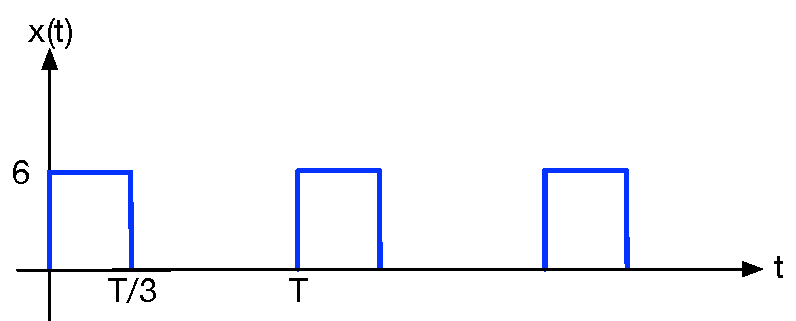
\includegraphics[width=6cm]{./Figuras/Problema3_3a}\end{figure*}}
	
	The resulting signal AM modulates a $125 V$ carrier, with a modulation index of $0.7484$. This signal is transmitted by a radio station. The transmission channel introduces 80 dB attenuation, and Gaussian white noise whose power spectral density is $N_0/2=10^{-11} W/Hz$.

	A vehicle is tuned to this radio station, and it enters a tunnel where the propagation attenuation is no longer constant and varies according to:

\begin{displaymath}
	A[dB] = a_0 + a_1 \cdot d
\end{displaymath}

where:
\begin{itemize}
	\item $a_0 = 10dB$
	\item $a_1 = \frac{1}{3} dB/m$
	\item $d$: Distance (m)
\end{itemize}

{\begin{figure*}[h!]\centering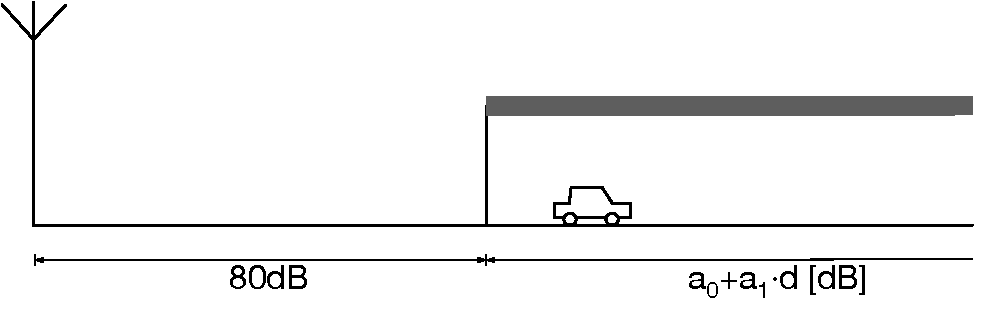
\includegraphics[width=8cm]{./Figuras/Problema3_3b}\end{figure*}}

	\begin{enumerate}
		\item Calculate the average power of the modulated signal.
		\item Calculate the demodulation signal-to-noise ratio at the tunnel entrance.
		\item Calculate the distance where the signal will no longer be audible, if the demodulation threshold is $10 dB$.
		\item Repeat c. when the demodulator employed is an envelope detector, assuming that the pre-detection threshold is $13 dB$.
	\end{enumerate}
	
}
{
\begin{enumerate}
	\item $S_T = 10kW$
	\item $\left ( \frac{S}{N} \right)_D = 20.38 dB$
	\item $d = 11.94m$
	\item $d' = 2.94m$
\end{enumerate}

}




\Problema{

	En un sistema de comunicación en el que la señal que llega al receptor tiene una potencia que está 100 dB por debajo de la potencia radiada por el transmisor y la densidad espectral de potencia de ruido es  $N_0/2=5\cdot 10^{-15} W/Hz$, se requiere una relación señal-ruido de demodulación superior a $40 dB$, para que la escucha sea correcta.
	
	El valor de la tensión máxima del mensaje es de $2 V$, su potencia media es de 1 vatio y su ancho de banda $10 kHz$. Obtener la potencia de transmisión mínima si se emplean los siguientes sistemas de modulación, considerando una relación señal a ruido en predetección umbral de $10 dB$:
	
	\begin{enumerate}
		\item Modulación DBL.
		\item Modulación AM, con $m=0.5$ y detector de envolvente.
		\item Modulación FM sin deénfasis ($f_d=10^5 Hz/V$).
	\end{enumerate}

}
{
	\begin{enumerate}
		\item $S_T = 10kW$
		\item $\gamma > \gamma_{th} \Rightarrow S_T = 170kW$
		\item $\gamma < \gamma_{th} \Rightarrow S_T = S_{T_{th}} = 420W$
	\end{enumerate}
	
}
{

	A communication system is such that the signal arriving at the receiver side has a power $100 dB$ below the emitted power at the transmitter side, and that the noise power spectral density is $N_0/2=5\cdot 10^{-15} W/Hz$. A post-detection signal-to-noise ratio of $40 dB$ is required for a correct reception.

The maximum voltage value of the message is $2 V$, its mean power is $1 W$, and its bandwidth, $10 kHz$. A pre-detection threshold signal-to-noise ratio of $10 dB$ is required. Calculate the minimum transmitted power when using each one of the following modulation systems:
	
	\begin{enumerate}
		\item DSB modulation.
		\item AM modulation with $m=0.5$ and envelope detection.
		\item FM modulation without de-emphasis ($f_d=10^5 Hz/V$).
	\end{enumerate}

}
{
	\begin{enumerate}
		\item $S_T = 10kW$
		\item $\gamma > \gamma_{th} \Rightarrow S_T = 170kW$
		\item $\gamma < \gamma_{th} \Rightarrow S_T = S_{T_{th}} = 420W$
	\end{enumerate}
	
}

\Problema{

	Se desea transmitir una señal de ancho de banda $10 kHz$ y potencia media normalizada de $0.5W$, a través de un sistema de comunicación FM. La relación señal a ruido de demodulación debe estar por encima de $40 dB$ con un mínimo gasto de potencia, para ello, se dispone de un canal cuyo ancho de banda es de $120 kHz$ y que introduce ruido blanco cuya densidad espectral de potencia es de $N_0/2=0.5\cdot 10^{-8} W/Hz$ y una atenuación de $40 dB$. Indicar cuál debe ser la potencia necesaria para transmitir la señal.
}
{
\begin{itemize}
	\item $S_T = 416.66 W$
\end{itemize}


}
{

	We want to transmit a signal with bandwidth $10 kHz$ and normalized average power $0.5$, by using an FM communication system. The post-detection signal-to-noise ratio has to be greater than $40 dB$, but ensuring a minimum amount of output power consumption. The channel has $120 kHz$ bandwidth and introduces white noise with power spectral density $N_0/2=0.5\cdot 10^{-8} W/Hz$. This channel is characterized by an attenuation of $40 dB$. Indicate the amount of power needed to trasmit the signal.
	
}
{
\begin{itemize}
	\item $S_T = 416.66 W$
\end{itemize}


}

\newpage

\Problema{

	Un sistema de transmisión por radio utiliza un modulador de frecuencia (FM) cuya constante del modulador es $f_d = 20 kHz/V$ y portadora $p(t)=5\cdot cos(2\pi \cdot 5\cdot 10^7 t)$. Se pide:
	
	\begin{enumerate}
		\item Calcular el índice de modulación D y el ancho de banda aproximado cuando la señal moduladora es $x_1(t) = cos(2\pi \cdot 500 t)$.
		\item Repetir el apartado anterior si la señal moduladora es $x_2(t)=cos(2\pi \cdot 10^4 t)$.
	\end{enumerate}
	

Para mejorar la relación señal-ruido de demodulación del sistema, se introducen unos filtros de preénfasis y deénfasis con frecuencia de corte $1430 Hz$ y se prueba el sistema con la señal moduladora $x(t) = x_1 (t) + x_2 (t)$.

\begin{enumerate}\setcounter{enumi}{2}
	\item Determinar la mejora en la relación señal-ruido de demodulación.
\end{enumerate}

}
{
\begin{enumerate}
	\item $D_1 = 40$, $B_T = 41kHz$
	\item $D_2 = 2$, $B_T = 80kHz$
	\item $\Delta \left ( \frac{S}{N} \right)_D = 12.14 dB$
\end{enumerate}

}
{

	A radio transmission system uses a frequency modulator (FM) with modulator constant $f_d = 20 kHz/V$, and carrier signal $c(t)=5\cdot cos(2\pi \cdot 5\cdot 10^7 t)$. Answer:
	
	\begin{enumerate}
		\item Calculate the modulation index D and the approximate bandwidth when the modulating signal is $x_1(t) = cos(2\pi \cdot 500 t)$.
		\item Repeat a. when the modulating signal is $x_2(t)=cos(2\pi \cdot 10^4 t)$.
	\end{enumerate}


In order to improve the demodulation signal-to-noise ratio, a pre-emphasis and de-emphasis filters are introduced, with cut-off frequency $1430 Hz$. The system is tested with the modulating signal $x(t) = x_1 (t) + x_2 (t)$.

\begin{enumerate}\setcounter{enumi}{2}
	\item Determine the improvement in demodulation signal-to-noise ratio.
\end{enumerate}

}
{
\begin{enumerate}
	\item $D_1 = 40$, $B_T = 41kHz$
	\item $D_2 = 2$, $B_T = 80kHz$
	\item $\Delta \left ( \frac{S}{N} \right)_D = 12.14 dB$
\end{enumerate}

}




\Problema{

	Hallar la relación señal ruido de postdetección en un sistema de transmisión por radio que utiliza un modulador de frecuencia (FM) y una moduladora $x(t)$ de ancho de banda es de $5 kHz$. y potencia media $0.5 W$ cuya amplitud varía entre $-1$ y $2V$. La desviación máxima de frecuencia es de $20 kHz$ y la potencia de la onda FM en el receptor es de $50 nW$. transmitiendo por un canal AWGN cuya densidad espectral de potencia de ruido es $N_0/2 = 3\cdot 10^{-14} W/Hz$.
}
{
\begin{itemize}
	\item $\left ( \frac{S}{N} \right )_D = 30dB$
\end{itemize}

}
{

	A signal with bandwidth $5 kHz$, whose maximum voltage value is $2 V$ and with average power $0.5 W$ is transmitted using FM through an AWGN channel. The channel has a noise power spectral density of $N_0/2 = 3\cdot 10^{-14} W/Hz$. The receiver power is $50 nW$. The maximum deviation of frequency is $20 kHz$. Calculate the post-detection signal-to-noise ratio.
}
{
\begin{itemize}
	\item $\left ( \frac{S}{N} \right )_D = 30dB$
\end{itemize}

}

\newpage


\Problema{

	Una señal de ancho de banda $10 kHz$ y potencia media normalizada $0.5$, se transmite en FM por un canal AWGN cuya densidad espectral de potencia de ruido es $N_0/2=5\cdot 10^{-10} W/Hz$ y que introduce una atenuación de $40 dB$. Para un correcto funcionamiento del enlace, el sistema requiere una $\gamma_{th}$ (umbral) de $100$ para una relación señal ruido predetección umbral de $10 dB$. Determinar:
	
	\begin{enumerate}
		\item La potencia de transmisión mínima ($S_T$).
		\item La relación señal ruido postdetección.
	\end{enumerate}

Con el fin de mejorar la relación señal a ruido en postdetección se introducen los correspondientes filtros de preénfasis y deénfasis, con $B_{de} = 1 kHz$.

\begin{enumerate}\setcounter{enumi}{2}
	\item Determinar la mejora en dB que experimenta la relación señal a ruido en postdetección.
\end{enumerate}

}
{
\begin{enumerate}
	\item $S_{T_{min}} = 10dBW$
	\item $\left ( \frac{S}{N} \right )_D = 31.3 dB$
	\item $\Delta \left ( \frac{S}{N} \right )_D = 15.23 dB$
\end{enumerate}
}
{

	A signal with bandwidth $10 kHz$ and normalized average power $0.5$ is transmitted using FM through an AWGN channel. The channel has a noise power spectral density of $N_0/2=5\cdot 10^{-10} W/Hz$ and attenuates the signal $40 dB$. In order to meet the required quality specifications, a threshold $\gamma_{th}$ of $100$ is required for a pre-detection threshold signal-to-noise ratio of $10 dB$. 

	\begin{enumerate}
		\item Calculate the minimum possible power transmitted to the channel ($S_T$).
		\item Find the demodulation (post-detection) signal-to-noise ratio.
	\end{enumerate}
	 
In order to improve the demodulation signal-to-noise ratio, pre-emphasis and de-emphasis filters are introduced. The $3 dB$ cutoff frequency of the de-emphasis filter, $B_{de}= 1 kHz$.

\begin{enumerate}\setcounter{enumi}{2}
	\item Determine the improvement in dB of the demodulation (post-detection) signal-to-noise ratio.
\end{enumerate}

}
{
\begin{enumerate}
	\item $S_{T_{min}} = 10dBW$
	\item $\left ( \frac{S}{N} \right )_D = 31.3 dB$
	\item $\Delta \left ( \frac{S}{N} \right )_D = 15.23 dB$
\end{enumerate}
}




\begin{thebibliography}{100}
	\bibitem[Carlson2010]{Carlson} A. Bruce Carlson and Paul B. Crilly. Communication Systems: An Introduction to Signals and Noise in Electrical Communication, 5th Ed. McGraw-Hill, 2010.
	%\bibitem[Haykin2001]{Haykin}  Simon Haykin. Communication Systems, 4th Ed. John Wiley and Sons, 2001.
	\end{thebibliography}
	
	

\end{document}



	
